\documentclass[a4paper,11pt]{article}

\usepackage[latin1]{inputenc}

\usepackage{tikz}
\usetikzlibrary{automata,arrows,topaths}


\newcommand{\nnsection}[1]{
\section*{#1}
\addcontentsline{toc}{section}{#1}
}

\begin{document}

\begin{center}
\vspace{20pt}
\textbf{\large An Erlang ray tracer}\\
\vspace{10pt}
\textbf{Johan Montelius}\\
\vspace{10pt}
\today{}
\end{center}

\nnsection{Introduction}

The goal of this assignment is that your should practice representing
data using tuples and records and, understand how a program can be
divided into modules to implement abstract data structures.

This is also an exercise in how to model a complex system and refresh
your knowledge of vector arithmetic. Hopefully it's also quite fun to
see how you can create your own images of a three dimensional world.

\section{A ray tracer}

In order to explain a ray tracer in a three dimensional world, we will
describe all necessary steps using a two dimensional model. Since we
will describe everything using vector arithmetic it can easily be
extended to a three dimensional model. Images generated in a two
dimensional world will of course not be very thrilling but we will be able to describe the necessary steps.

In Fig.~\ref{fig:world} we see a sphere in a two dimensional Cartesian
coordinate system. A {\em camera} is also positioned in the room
consisting of a {\em canvas} and an {\em eye}. When generating an
image we need to trace as many rays as possible starting in the eye of
the camera and passing through the {\em pixels} of the canvas. If we
can determine that a ray intersect with an object we can color the
pixel thus generating an image on the canvas.


\begin{figure}[ht]
\centering  
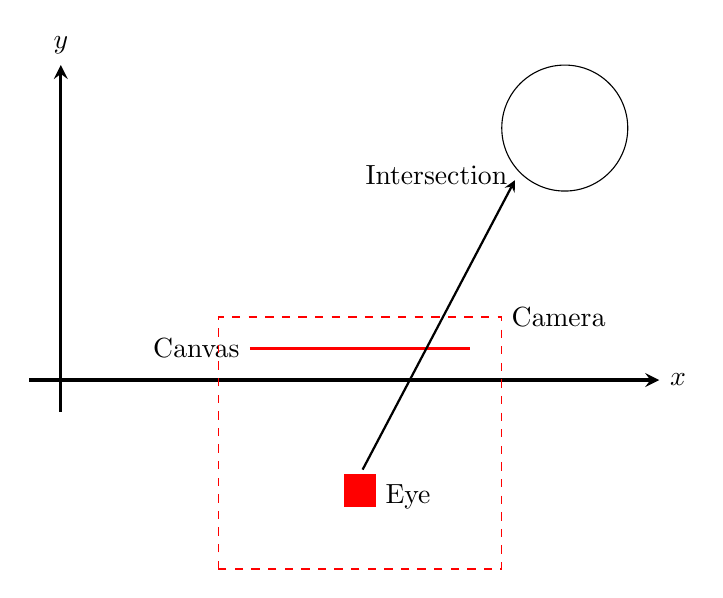
\begin{tikzpicture}[
        scale=0.4,
        axis/.style={very thick, ->, >=stealth},
        important line/.style={thick},
        dashed line/.style={dashed, thin},
        pile/.style={thick, ->, >=stealth, shorten <=2pt, shorten >=2pt},
        every node/.style={color=black}]

    % axis
    \draw[axis] (-1,0)  -- (19,0) node(xline)[right] {$x$};
    \draw[axis] (0,-1) -- (0,10) node(yline)[above] {$y$};

    \draw (16,8) circle (2);

    \filldraw[red] (9,-4) rectangle (10,-3) node(eye)[below right]{Eye};
    \draw[red, thick] (6,1) node(canvas)[left] {Canvas} -- (13,1);
    \draw[red, dashed] (5,-6) rectangle (14,2) node(camera)[right]{Camera};
    \draw [pile] (9.5,-3) -- (14.5,6.5) node(hit)[left]{Intersection}; 
\end{tikzpicture}
\label{fig:world}
\caption{A model of the world.}
\end{figure}

The beauty of vector arithmetic is that if we understand how to do the
necessary calculations in a two dimensional space then we also know
how to do it in a three dimensional space. If we extend this model to
a three dimensional world, we would have a sphere instead of a circle
and the canvas would be a rectangular plane. The eye would still be a
point in this space and we would track rays from the eye through each
{\em x-y pixel} of the canvas.

To model our world and do the necessary computations we need to solve
the following problems:

\begin{itemize}
 \item represent and do calculations on vectors
 \item represent objects such as spheres
 \item represent rays
 \item determine if a ray intersects an object
 \item represent a camera i.e. the location of the eye and the canvas
\end{itemize}

When we solve these problems we will try to separate them as much as
possible form each other. We will divide our system into modules were
each module is responsible for one sub-problem or abstraction. If we do
it right the main program can describe operations in a much higher
level; instead of talking about x, y and z coordinates it can talk
about rays, objects and intersections.


\section{Vectors}

The first task is to create a module that will handle all vector
operations. We will need to represent vectors and be able to do the
following operations.

\begin{itemize}
 \item $a\vec{x}$ : scalar multiplication
 \item $\vec{x} - \vec{y}$ : subtraction
 \item $\vec{x} + \vec{y}$ : addition
 \item $\|\vec{x}\|$ : norm, or length, of a vector
 \item $\vec{x} \cdot \vec{y}$ : scalar product (dot product)
 \item $|\vec{x}|$ : normalized vector
\end{itemize}

If we restrict the system to only work with three dimensional vectors
we have a natural way of representation: a tuple with three elements,
the $x$, $y$ and $z$ components i.e. {\tt \{X, Y, Z\}}. 

Create a new file {\tt vector.erl} and declare a new module with the
following exported functions.

\begin{verbatim}
-module(vector).
-export([smul/2, add/2, sub/2, norm/1, normalize/1, dot/2]).
\end{verbatim}

The first functions, scalar multiplication, addition and subtraction
should be quite easy to implement.

$$\langle x_1, x_2, x_3 \rangle  s =  \langle x_1s, x_2s, x_3s \rangle$$

$$\langle x_1, x_2, x_3 \rangle + \langle y_1, y_2, y_3\rangle = \langle x_1+y_1, x_x+y_2, x_3+y_3 \rangle$$

To implement the norm, dot product and normalization of a vector you
might have to go through your book in linear algebra but you should
have it up and running quite quickly.

$$\|\vec{x}\| = \sqrt{x_1� + x_2� + x_3�}$$

$$ \vec{x} \cdot \vec{y} = \langle x_1*y_1 + x_2*y_2 + x_3*y_3\rangle $$ 

$$ |\vec{x}| = \vec{x}/\|\vec{x}\|$$

In this implementation we actually expose the representation of a
vector i.e. the users of this module will know that vectors are
represented by tuples with three elements. This is not the best
solution but unfortunately a very convenient solution.

\section{objects}

Our next task is to create a module that can represent the objects in
our world. We will keep things simple and only handle rays and
spheres. 

When we decide on the representation we need to think about the
operations we should perform; a representation is efficient if it
allows the operations to be efficiently implemented. When we are
talking about rays and spheres, we might not have much choice but it's
important to start thinking about the operations that should be
performed.

The operations that we will perform over and over again is to
determine if a ray intersects with another object such as a sphere. If
we model our objects in a Cartesian space we will be able to
determine intersections quite easily. A ray will have an origin and a
sphere will have an origin and a radius. An origin is represented by
a vector, a direction by a normalized vector and a radius by an integer.

When we choose a representation of rays and spheres we will use Erlang
records. Records are very similar to tuples but they are identified by
a name and also have named elements. We will later add more properties
to these objects and the record structure makes it much easier to
modify our code.

\begin{verbatim}
-module(obects)

-record(ray, {origin, direction}).

-record(sphere, {radius, center}).

-export([ray/2, sphere/2, intersect/2]).
\end{verbatim}

The first two functions will simply return objects of specified
types. You see how we use the record constructs and initiate the named
elements. 

\begin{verbatim}
ray(Origin, Direction) ->
    #ray{origin=Origin, direction=Direction}.

sphere(Radius, Center) ->
    #sphere{radius=Radius, center=Center}.
\end{verbatim}

The tricky part is of course to determine if a ray will intersect a
sphere but this is actually easily determined if we remember our linear algebra.


\begin{figure}[ht]
\begin{center}
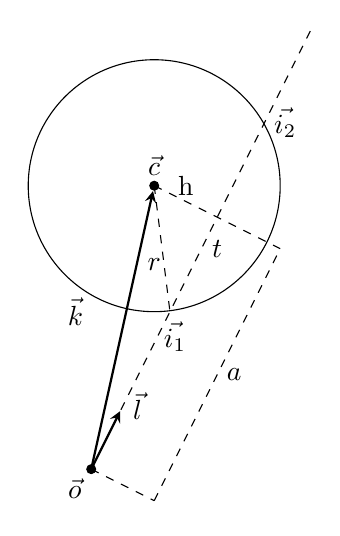
\begin{tikzpicture}[
        scale=0.4,
        important line/.style={thick},
        dashed line/.style={dashed, thin},
        pile/.style={thick, ->, >=stealth, shorten >=2pt},
        every node/.style={color=black}
    ]
    \draw[fill] (6,6) node()[above]{$\vec{c}$} circle (4pt);
    \draw (6,6) circle (4);

    \draw[fill] (4,-3) node()[below left]{$\vec{o}$} circle (4pt);

    \draw [dashed](4,-3) -- (11,11); 

    \draw [thick,pile](4,-3) -- (5,-1) node(l)[right]{$\vec{l}$};  

    \draw  (6,2) node(i1)[below right]{$\vec{i_1}$};
    \draw  (9.5,8) node(i2)[right]{$\vec{i_2}$};

    \draw [thick, pile] (4,-3) -- (6,6);
    \draw (3.5,2) node(k)[]{$\vec{k}$};

    \draw[dashed] (6,6) -- (6.5,2);
    \draw (6,3.5) node(){$r$};

    \draw[dashed] (6,6) -- (10,4);  %% (4, -2)
    \draw (7,6) node[]() {h};

    \draw[dashed] (4,-3) -- (6,-4);   %% (2,-1)

    \draw[dashed] (6,-4) -- (10,4) node()[midway, right] {$a$};

    \draw (8,4) node(){$t$};

\end{tikzpicture}    
\caption{Intersection of ray and sphere.}
\label{fig:intersection}
\end{center}
\end{figure}

In Fig.~\ref{fig:intersection} we see a ray intersecting a circle. We
want to find the intersection points $\vec{i_1}$ and $\vec{i_1}$.We
can do this by first calculate the length $a$ and this is done by taking
the dot product of $\vec{k}$ and $\vec{l}$. The dot product will
project the vector $\vec{k}$ on $\vec{l}$ thus giving us the
length $a$. The vector $\vec{k}$ is of course easily calculated since we
know the origin of the ray $\vec{o}$ and the center of the circle
$\vec{c}$.

Note that we here talk about the circle while our real model would
contain a sphere - this is fine, the operations are the same.


The length of the vector $\vec{k}$ is of course $\|\vec{k}\|$
and if we know this we can calculate $h$
using Pythagoras' theorem. Since we know that the radius of the
sphere is $r$ we can again rely on Pythagoras and calculate $t�$.

$$ t� = r� - h� $$

If it turns out that $t�$ is a negative value, it means that the ray
does not intersect the sphere. This is our criteria for answering if
we intersect the object or not. If $t�$ is positive we calculate $t$
and then of course obtain two alternatives $t$ and $-t$.  We now
calculate two distances $d_1 = a - t$ and $d_2 = a + t$.  This is the
distance to the points of intersections from the origin of the ray
$\vec{o}$.  If either value is negative it means that the intersection
point is behind us; if only one value is negative we are actually
inside the sphere. If both values are positive we return the smallest
value since this is the surface that we will actually see.

Implement the function {\tt intersection/2} that checks if ray
intersects a sphere; return {\tt no} if it does not and {\tt \{ok,
  D\}}, where {\tt D} is the closest distance, if it does. Do some
experiments to see that it works.

\begin{verbatim}
intersect(#sphere{radius=R, center=C}, 
          #ray{origin=O, direction=L}) ->
      :
      :
\end{verbatim}

\section{the camera}

We have now done half of the job, you will soon create your first
image but we first need to represent the camera. It turns out that we
have a lot of options when defining what the camera looks like; we of
course need to define where in the room it is and where it is pointing
but also what kind of lens it has. This is probably the most
complicated part of the implementation but we will give it a try.

\subsection{the name of the game}

In the end we would like to have a representation of a camera that
will allow us to ask for a ray that starts in the focal point (or
origin) of the camera and runs through a given $\langle x, y\rangle$
coordinate of the canvas. If we know that the canvas is of size
$800 \times 600$
then we can ask for the ray that runs through
$\langle 230, 170\rangle$
and be given a a ray. This ray will then be compared to all the
objects in the world and the closest intersection point will determine
the color of the $\langle 230, 170\rangle$ pixel.

When you think about representation, then always think about what
you're going to use the object for. This will allow you to represent
the object in a way that makes the operations easier to perform. Also
think about how you would like to talk about the object, the easiest
way to describe an object might not be the bets way to represent it.

\subsection{properties of a camera}

If you have not used a large camera you might not have thought about
how different lenses changes the picture but think about the
difference between a ``fish-eye'' and telephoto lens. The difference
has to to with the {\em focal length}, the length from the lens to the
focal point; the important factor is the ratio between the width of
the {\em film} and the focal length. When using a 35mm film a focal
length of 50mm gave a ``normal'' lens i.e. a lens that gave images
that looked normal.

It is thus important that we can describe a {\em canvas}: its size,
orientation and position in relation to the {\em origin} of the
camera. In Fig.~\ref{fig:camera} we see the elements that we need to
represent: the origin described by a vector $\vec{o}$,
a vector $\vec{f}$
that give us the direction and distance to the center of the canvas
and two vectors that give us the vertical, $\vec{v}$,
and horizontal, $\vec{h}$,
direction of the canvas. 

We might take for granted that the plane of the canvas is orthogonal to
the direction; this is not strictly necessary but if it is not, we will
have very strange projections of the image (a technique that is
actually used and if you want to know more you can search for the
``Scheimpflug principle'').

Note that the vertical and horizontal orientation are represented as
two vectors. This will allow us to create a ray from the origin through
any coordinate of the canvas. 

\begin{figure}[ht]
\begin{center}
\begin{tikzpicture}
\draw[fill] (0,0,0) node()[left]{$\vec{o}$} circle (2pt);

\draw[->] (0,0,0) -- (4,4,4) node()[below, near start]{$\vec{f}$};

\draw[->] (4,4,4) -- ++(0,2,0) node()[right, midway]{$\vec{v}$};

\draw[->] (4,4,4) -- ++(3,0,3) node()[below, midway]{$\vec{h}$};

\draw[dashed] (7,6,7) -- (7,2,7) -- (1,2,1) -- (1,6,1) -- cycle;

\end{tikzpicture}
\caption{Representing a camera.}
\label{fig:camera}
\end{center}
\end{figure}

A camera with a normal lens, positioned at $\langle 0,0,0\rangle$
and pointing straight into the picture, could be described as follows:

\begin{itemize}
 \item position: $\langle 0,0,0\rangle$
 \item direction: $\langle 0,0,1200\rangle$
 \item horizontal: $\langle 960,0,0\rangle$
 \item vertical: $\langle 0,540,0\rangle$
\end{itemize}

This would give us a canvas of size $1920 \times 1080$
at a distance from the origin of $1600$ (which will approximately give us a ``normal'' lens). 

To minimize the computation needed when calculating the rays we could
represent the camera by a position and a vector to the upper left
corner of the canvas $\vec{c}$. If we then have two vectors that represent the
distance between pixels moving to the right $\vec{r}$ and moving down $\vec{d}$, we can
easily calculate the normalized vector to any pixel in the canvas.

$$pixel(x,y) = |\vec{c} + x*\vec{r} + y*\vec{d}|$$

We therefore represent the camera by position, direction to the upper
left corner and the two vectors that describes the distance to the
first pixel to the right and the first pixel down. Why the upper
corner, why move down, why not lower left corner? Turns out that when
we talk about images we often count the rows going down so this will
makes things easier. We also keep the size of the canvas so we know
which rays that we should produce.

Open up a module {\tt camera} and defined the following record. 

\begin{verbatim}
-record(camera, {pos,    % the position of the camera
                 corner, % the upper left corner
                 right,  % the vector going right
                 down,   % the vector going down
                 size    % the {width, height}
                }).
\end{verbatim}

You should also define, and export, a function {\tt camera/5} that will
return a camera given the properties. It will also be very handy to
have a function that returns a default camera so that we don't have to
think about the different parameters. This default camera can be
positions at $\langle 0,0,0\rangle$
and point straight forward (in the z direction). We can give it a
parameter that is the size of the image that we want to generate; you
will have to calculate the rest of the parameters.

\begin{verbatim}
camera(Pos, Corner, Right, Down, Size) ->
    #camera{pos = Pos, corner = Corner, 
            right = Right, down = Down, size = Size}.

normal(Size) ->
    {Width, Height} = Size,
    D = Width * 1.2,  % aprx normal lens
    H = Width / 2,
    V = Height /  2,
    Corner = ...
    camera({0,0,0}, Corner, ..., ..., Size).
\end{verbatim}

Given a camera we now need to calculate a ray that passes through a
given coordinate or pixel. This should be straight forward given that
we created our representation with this mind.

\begin{verbatim}
ray(X, Y, Camera) ->
    Origin = ...   % the origin of the ray
    Xpos = ...     % a vector from the corner to the X column
    Ypos = ...     % a vector from the corner to the Y row
    Pixle =  ...   % a vector from origin to the pixle
    Dir =  ..      % the normalized vector
    objects:ray(Origin, Dir).
\end{verbatim}

Also implement a function {\tt size/1} that returns the size of a
camera and then you're done with the camera module.

\section{the world}

The world is simply a list of objects. We will extend the world to also
hold other things but for our first test this will be sufficient.

\begin{verbatim}
-module(world).

-export([world/1]).

-record(world, { objects=[] }).

world(Objects) ->
    #world{objects=Objects}.    
\end{verbatim}

That completes all the modules that we need, high time to generate some images. 

\section{the tracer}

Open a module called {\tt tracer}; this will be the main module where
the images are created. We will define a function that takes a camera
and a description of the world and returns an image.

An image will be represented by a list of rows where each row is a
list of {\em rgb values}. The rgb values are tuples of three elements
where each element is a floating point value between $0$ and $1$. A
green-blue color could thus be represented by the tuple {\tt \{0, 0.8,
  0.3\}} We will later use a procedure to print this image to a file
that you hopefully can open in a viewer of your choice.

We will start slowly and render a black and white image. This will not
impress anyone but your mother, but it will be a start that we then
will extend quite easily. We will build the tracer {\em bottom up}
which will give us the opportunity to test things as we implement
it. 

The first thing we will do is to determine which object a ray
intersects, if any, from a list of objects. We know that we can call
{\tt intersect/2} form the {\tt objects} module but now we have a list
of objects and we want to find the closest point of intersection. 

The {\tt intersect/2} function returns either {\tt \{ok, D\}} or {\tt
  no} so it should be an easy task to find the object with the closest
point of intersection. We will here use the higher order construct
{\tt foldl/3} but you could implement it by hand in just as many lines. 

\begin{verbatim}
intersect(Ray, Objs) ->
   lists:foldl(fun(Obj, Sofar) -> 
                       {Dist, _} = Sofar,
                       case objects:intersect(Obj, Ray) of
                           {ok, D} when D < Dist ->
                               {D, Obj};
                           _ ->
                               Sofar
                       end
               end,
               {inf, no},
               Objs).
\end{verbatim}

So the function {\tt intersect/2} will tell us if a ray intersects an
object and it will also tell us the distance to this object. If the
ray does not intersect an object it will return {\tt \{inf, no\}}
(using a value like this is called a sentinel, a value that we know
will be higher than any other value).

We now define a two functions: {\tt trace/4} and {\tt trace/2}. The
latter will use {\tt intersect/2}, check the outcome and then return
either a black or white rgb-value depending on if we intersected an
object. The first will use the latter but here we give the x and y
values of the pixel that we are looking for,

\begin{verbatim}
-define(Black, {0,0,0}).
-define(White, {1,1,1}).

trace(X, Y, Camera, Objects) ->
    Ray = ...
    trace(Ray, Objects).

trace(Ray, Objects) ->
    case intersect(Ray, Objects) of
        ... ->
            ?Black;
        ... -> 
            ?White
    end.
\end{verbatim}

The only thing that is left is to trace every possible ray of the
camera; this is neatly done using list comprehension. The function
{\tt tracer/2} will return a list of rows where each row is a list of
rgb values that describes the image.

\begin{verbatim}
tracer(Camera, Objects) ->
    {W, H} = camera:size(Camera),
    Xs = lists:seq(1, W),
    Ys = lists:seq(1, H),
    [[trace(X, Y, Camera, Objects) || X <- Xs] || Y <- Ys].
\end{verbatim}

\section{an image}

We of course want to look at the image we have created and to do this
we somehow have to convert it into a image file. There are many image
formats to choose from but most are compressed and it is not trivial
to write a jpeg encoder. The file format that we will use is very
inefficient but it is very easy to generate a file. In the appendix
App~\ref{app:ppm} you will find a module that will take an image, as we
generates it, and writes a {\em ppm} file. Not all image viewers can
open a ppm file so you might have to try several before finding one that works.

It is now quite easy to generate an image, all we have to do is to describe the world and then take a snap shot. Create a module called {\tt test} and describe your first image.

\begin{verbatim}
-module(test).

-compile(export_all).

snap(0) ->
    Camera = camera:normal({800,600}),
    Obj1 = objects:sphere( 140, {    0,    0, 700}),
    Obj2 = objects:sphere(  50, {  200,    0, 600}),
    Obj3 = objects:sphere(  50, {  -80,    0, 400}),
    World = [Obj1, Obj2, Obj3],
    Image = tracer:tracer(Camera, World),
    ppm:write("snap0.ppm", Image).
\end{verbatim}

If you look at your picture you will hopefully see three white circles
on a black background. One circle (the image of {\tt Obj3} in the
description above) is closer to the camera and is partly blocking the
larger circle (that is the image of {\tt Obj1}). This is not very
existing but you will see that it is very easy to extend this simple ray tracer. 

\section{extensions}

We will do three extensions to the tracer: colors, lights and
reflections. The first extension is quite simple while the last one
requires that you repeat you knowledge i geometry. 

\subsection{adding colors}

Turning the image into a color image is two simple changes. First of
all we extend the {\tt sphere} record structure to also include a
color element. We can have a default color if we want so that all
spheres have colors; we also provide a function {\tt sphere/3} that
will create colorful spheres.

\begin{verbatim}
-define(Color, {1.0,0.4,0.4}).

-record(sphere, {radius=2, center, color=?Color}).

sphere(Radius, Center, Opt) ->
    Color = case lists:keyfind(color, 1, Opt) of
                {color, C} ->
                    C;
                false ->
                    ?Color
            end,
    #sphere{radius=Radius, center=Center, color=Color}.

color(#sphere{color=Color}) ->  Color.
\end{verbatim}

The way we choose to implement {\tt sphere/3} is a bit over-kill but we
now have a simple way of adding more properties as we go (and we
will).

Once we have spheres with colors, we simply change the {\tt trace/3}
function so that it will return the color of the object rather than
the default white. Describe a new snap-shot where you have some
colorful spheres and see what the image looks like.

\subsection{lights}



We will do two things in this extension; we will introduce a
world-object that holds general information about the world and then
we will add lights. Create a module called {\tt world} and
describe a world object:

\begin{verbatim}
-define(Bkg, {0.0,0.0,0.0}).

-record(world, { objects=[], lights=[], background=?Bkg }).

world(Objects, Lights, Opt) ->
    Bkg = case lists:keyfind(background, 1, Opt) of
                {background, B} ->
                    B;
                false ->
                    ?Bkg
            end,
    #world{objects=Objects, lights=Lights, background=Bkg}.
\end{verbatim}

We use the same scheme as for the spheres and have a function that can
create a world given a list of objects, a list of lights and an list
of additional properties. One of the properties we will add right now
is the background color.

The question is now what a light source looks like; we create a new
module {\tt light} that will handle all aspects of it. The lights
themselves are simple to model since we only give them a position and a
color.

\begin{verbatim}
-record(light, {origin, color={1.0,1.0,1.0}}).

light(Origin, Color) ->
    #light{origin=Origin, color=Color}.
\end{verbatim}

The question now is how we are going to use the lights; we could
probably have a whole course on how light sources are combined in a
ray tracer but we will try to keep it simple. 

Let's look at the trace function, it detects if a ray hits an object
and then returns the object and the distance to this object. Since we
know the direction of the ray we can easily describe the point in
space where the ray hits the object. Now what if we ask if a ray
starting in this point, in the direction of a light source, hits any
object in the world - if not the point should be illuminated by the
light source. If we examine all light sources we would determine which
sources that illuminates the point and combined with the color of the
object we can determine what the color of the corresponding pixel. Note
that you have all the pieces of this puzzle, it's just a matter of
combining light sources and the color of the object.

\begin{verbatim}
trace(Ray, World) ->
    Objs = world:objects(World),
    case intersect(Ray, Objs) of
        {inf, _} ->
            world:background(World);
        {D, Obj} -> 
            O = objects:origin(Ray),
            L = objects:direction(Ray),
            I = vector:add(O, vector:smul(L, (D-?Delta))),
            Visible = visible(I, world:lights(World), Objs),
            Normal = objects:normal(I, Obj),
            Illumination = lights:combine(I, Normal,  Visible),
            lights:illuminate(Obj, Illumination, World)
    end.
\end{verbatim}

In the code above there are two things that needs some explanation:
the {\tt ?Delta} and the use of the {\em normal vector}. The delta is
a hack that we need to do since floating points are not exact, or
rather since a point that is actually ``in'' the surface of an object
might be shadowed by the object it self. By raising the point a small
distance from the surface we avoid being lured into thinking that we
are in the surface or even worse below the surface; the delta that I
use is $0.001$ and it works fine.

The second thing is the normal vector that we calculate use when
combining the light sources. A light that hits the surface at an angle
will contribute to less illumination compared to a light that hits it
straight from above. You can first try to combine the light sources
without taking this into effect but you will see that the light is
very sharp, either it illuminates the surface or it does not. Using
the normal vector does require that you do some more vector
arithmetic but it turns out to be quite simple.

The normal vector $\vec{n}$ is easily calculate since we know the point
of intersection $\vec{i}$ and the center of the sphere $\vec{c}$. If
we have other objects we would of course have to do something else.

$$ \vec{n} = |\vec{i} - \vec{c}| $$

The contribution $a$ of a light source at $\vec{s}$ to the point
$\vec{i}$ on a surface with normal vector $\vec{n}$ is:

$$a =  |\vec{s} - \vec{i}| \cdot \vec{n}$$

What we are doing here is to first calculate the vector from $\vec{i}$
to $\vec{s}$ and then normalize this. Then we do the dot product with
the normal vector to obtain a number between $0$ and $1$.  An light
source that is orthogonal to the normal vector will not contribute at
all while a light source in exactly the same direction will contribute
with its full strength.

All the light sources can be added together but we of course need to
do the addition in a special way. When you add two probabilities $p$
and $q$ then you would write:

$$ 1 - ((1-p) \times (1-q))$$

and we should do the same thing here (do some thinking). If you get it
right your images will get a lot more live and will start to look like
something that you could show to someone besides your mother.

\subsection{reflections}

The third extension that we will look at is reflections; sounds tricky
but it turns out to be even simpler than adding lights. What we wan to
do is to calculate a reflecting ray in the point of intersection and
then calculate the contribution from this angle. The contribution can
of course be calculated using a recursive step since this is exactly
what the tracer module will do; given a origin and a normal vector
calculate what is visible in this direction. 

So if we do a recursive step and find that the reflection has a
particular color then we need to ask ourselves how much of this color
should be added to the point of intersection. This is where you will
start to think about {\em brilliance} i.e. how much the surface acts as
a mirror. Again, you could spend the rest of the week thinking about
how a metal surface is different from wood but we might also just
describe the level of reflection by a number from $0$ to $1$.

Add a property to the sphere object that gives us the brilliance and
then use this value when you calculate how much the reflection should
be visible. You then modify the {\tt tracer/2} function so it takes
another argument which will be the depth, or number of reflections. If
the depth is zero we're done and simply return the background color,
otherwise we calculate the intersection point, calculate the
contribution from light sources and then also add the reflection that
you obtain from a recursive call to the function (remember to
decrement the depth value).

Once we have the brilliance we might want to change the way we add
light sources since a light source that is in the direction of the
reflection would be visible in a sphere with high brilliance. If you
start to dig into this you will find that you have enough to do for a
day or two.

\subsection{and more}

Another thing that we might want to explore is of course to add more
objects. A plane would be fairly easy to describe and the intersection
can be found if you do some reading.

We could also start to add texture or images to the surface of
objects. An image could of course be mapped to a rectangular plane or
cylinder and you would see the distorted photo in your rendered image.

A fairly simple thing to add is transparency; an object can be made to
look like colored glass. To do this you would simply calculate two
contributing rays at a point of intersection. One is in the direction
of the reflection but the other one is continuing through the object,
this is called the {\em refraction}. The refraction is of course, if
you remember what you learned in secondary school, slightly bent
depending on the index of the material. You would thus use the
refraction index to calculate the direction of the ray and then take
the transparency into account when you add the contribution of the
refraction.

\section{summary}

This tutorial was not about ray tracing but about how you can work
with tuples, records and modules to build a larger program where try
to hide the internal data representation as much as possible.

If you have programmed in for example Java, which is a statically typed
object orientated language, you have seen better ways of doing
this. The dynamically typed languages have for good and worse less
support to achieve this; the record construct in Erlang is a addition
to the language that gives you some support but it's only half way.

If your familiar with object orientated languages you have probably
thought about describing out objects in a hierarchical way; all object
have a position and color, spheres are object that have a radius
etc. This would definitely make our life easier but again, the dynamic
nature of Erlang makes it harder to provide.

When looking at you program you could see the different modules as the
building blocks of abstractions. If you have done it right only the
vector module knows how vectors are handled (all though we cheated
and anyone that creates an object must also know how a vector is
represented. Anything that is dealing with rays, objects and
intersections should be in the objects module and everything that
handles colors and lights should be in the light module. Dividing you
program up in modules gives you a similar tool for abstractions as the
classes in Java (not exactly by similar). Learning how to divide a
program into different modules of abstraction is maybe the most
important skill of a good programmer.

Even if the tutorial was not about ray tracing, I hope that you have
generated some nice images and have a better understanding of what
your graphic card is doing when you spawn in BF.

\newpage
\appendix
\section{module ppm.erl} \label{app:ppm}
\begin{verbatim}
-module(ppm).

-export([write/2]).

%%% write(Name, Image) The image is a list of rows, each row a list of
%%% tuples {R,G,B} where the values are flots from 0 to 1. The image
%%% is written using PMM format P6 and color depth 0-255. This means that
%%% each tuple is written as three bytes.

write(Name, Image) ->
    Height = length(Image),
    Width = length(hd(Image)),
    {ok, Fd} = file:open(Name, [write]),
    io:format(Fd, "P6~n", []),
    io:format(Fd, "#~s~n", ["generated by ppm.erl"]),
    io:format(Fd, "~w ~w~n", [Width, Height]),
    io:format(Fd, "255~n", []),
    rows(Image, Fd),
    file:close(Fd).

rows(Rows, Fd) ->
    lists:foreach(fun(R) -> 
                          Colors = row(R), 
                          io:put_chars(Fd, Colors) 
                  end, Rows).

row(Row) ->
    lists:foldr(fun({R,G,B}, A) -> 
                        %% convert to 0-255
                        [ trunc(R*255), trunc(G*255), trunc(B*255) | A] end, 
                [], Row).   



    Rows).
\end{verbatim}
\end{document}
